

\documentclass[review,3p,times,12pt,number]{elsarticle}\usepackage{amsmath}\usepackage{amssymb}




\usepackage{multicol,enumitem,multirow,booktabs,amsthm,subfigure,rotating}
\usepackage{pdflscape}


\newlength{\smalltable}
\setlength{\smalltable}{252pt}


\newtheorem{proposition}{Proposition}
\newtheorem{definition}{Definition}


\usepackage[vlined,ruled,linesnumbered]{algorithm2e}
\SetKwComment{tcp}{/\!/\,}{}
\SetArgSty{textrm}
\SetKwProg{Procedure}{procedure}{}{end~procedure}
\SetKwProg{Function}{function}{}{end~function}
\SetKwFor{Repeat}{repeat}{times do}{end~loop}
\SetKwFunction{Move}{Move}
\SetKwFunction{Relocate}{Relocate}
\SetKwFunction{EvalMove}{EvalMove}
\SetKwFunction{Valid}{ValidTasks}
\SetKwFunction{Largest}{LargestPriorityTasks}
\SetKwFunction{EvalTask}{EvalTask}
\SetKwFunction{MoveNeed}{MoveNeed}
\SetKwFunction{Fill}{Fill}
\SetKwFunction{BiReceiver}{BiReceiver}
\SetKwFunction{BiSender}{BiSender}
\SetKwFunction{Interim}{Interim}
\SetKwFunction{InterimFull}{InterimFull}
\SetKw{Break}{break~while}

\renewcommand{\citet}[1]{\citeauthor{#1}~\citep{#1}}
\makeatletter
\def\NAT@def@citea{\def\@citea{\NAT@separator}}
\makeatother

\usepackage[colorlinks=true]{hyperref}



\usepackage{caption}
\captionsetup[figure]{font=small}
\captionsetup[table]{skip=0.5ex,font=small}



\renewcommand{\gets}{\coloneqq}
\renewcommand{\emph}[1]{\textbf{\textit{#1}}}



\newcommand{\mss}{s^\mathrm{src}}
\newcommand{\mds}{s^\mathrm{dst}}
\newcommand{\mts}{s^\mathrm{tmp}}




\newcommand{\setalgo}{\linespread{1}\fontsize{10}{12}\selectfont}
\newcommand{\settab}{\linespread{1}\fontsize{10}{12}\selectfont}

\sloppy


\begin{document}

\begin{frontmatter}

\journal{EJOR}
\title{A feasibility-based heuristic for the container pre-marshalling problem}
\author[shu]{Ning Wang}
\ead{ningwang@shu.edu.cn}



\author[cityu]{Bo Jin\corref{cor}}
\ead{msjinbo@cityu.edu.hk}

\author[syu]{Zizhen Zhang}
\ead{zhangzizhen@gmail.com}

\author[nus]{Andrew Lim}
\ead{alim.china@gmail.com}
\cortext[cor]{Corresponding author.}

\address[shu]{Department of Information Management, School of Management, Shanghai University, Shanghai, China}
\address[cityu]{Department of Management Sciences, City University of Hong Kong, Hong Kong}
\address[syu]{School of Data and Computer Science, Sun Yat-Sen University, China}
\address[nus]{Department of Industrial \& Systems Engineering, National University of Singapore, Singapore}

\begin{abstract}

This paper addresses the container pre-marshalling problem (CPMP) which rearranges containers inside a storage bay to a desired layout.
By far, target-driven algorithms have relatively good performance among all algorithms; they have two key components: 1) containers are rearranged to their desired slots one by one in a certain order; and 2) rearranging one container (a task) is completed by a sequence of movements. Our paper improves the performance of the target-driven algorithm from these two components.
This paper determines the order of container rearrangement as the algorithm goes on by the concept of state feasibility, stability, dead-end avoidance and tier-protection.
In addition, we improve the efficiency of performing tasks by discriminating different task types.
Computational experiments showcase that the performance of our proposed heuristic is considerable.
\end{abstract}

\begin{keyword}
container pre-marshalling problem \sep feasibility-based heuristic \sep tier-protection
\end{keyword}
\end{frontmatter}




\section{Introduction}



Since the commencement of containerization, the global use of standardized containers has dramatically improved international trade. Containers enable the smooth flow of goods between multiple transportation modes without directly handling the freight. Over the years, stringent requirements from consignors such as just-in-time operations have created challenges for the container transportation industry.

Container yards --- the space dedicated to the transshipment, handover, loading, consolidation, maintenance, and storage of containers --- are key components of maritime container terminals. Some yards act as exchange venues for container transfers between different transportation modes while others are used as caches for temporary storage or as warehouses for long-term storage.

Generally speaking, a container yard is divided into several yard blocks, each of which consists of several parallel bays.  A bay is formed by a row of stacks. Usually the containers stored in the same bay have the same dimensions. Equipments such as rubber tyre gantry cranes, rail-mounted gantry cranes, and reach stackers are frequently used in container yards. Figure~\ref{fig:block} illustrates an example of a yard block.

\begin{figure}[htbp]
\centering
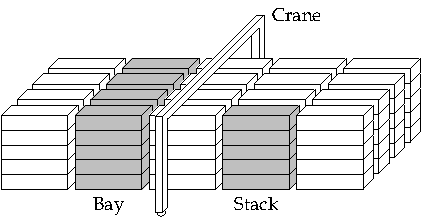
\includegraphics{figs/block.pdf}
\caption{Yard block.}
\label{fig:block}
\end{figure}

Containers in the same stack are organized in a last-in-first-out matter. To retrieve containers placed in lower levels, containers on top of them must be relocated to other slots or the yard first. Such forced movements are known as container reshuffles.
The container pre-marshalling problem~(CPMP) addresses the reorganization of containers inside a storage area such that no reshuffle is further required when containers are retrieved. Hence, the aim of CPMP is to improve terminals' performance level, including throughput rate per berth and the turnaround time of vessels or road trucks~\citep{kim2015}.

The CPMP can be formally defined as follows: containers marked with group labels are initially placed in a bay. The CPMP aims at rearranging these containers within the bay, so that containers in each stack are placed in a descending order of group labels from bottom to top. The objective is to carry out the rearrangement with the fewest number of container movements.
It is assumed that the retrieval order of the containers is known beforehand and no container arrives at or leaves from the bay during the pre-marshalling.

This paper designs a constructive heuristic which can be embedded later into frames such as beam search or GRASP\@.
Our work makes three main contributions to the literature.
One contribution is the concept of feasibility. We quantitatively find a necessary condition for a feasible instance.
The feasibility of rearranging a certain container is checked before we actually conduct the rearrangement, which guarantees the search efficiency.
The time complexity of checking the feasibility is only $\mathcal O(G)$; here $G$ is the number of groups. Our paper is the first work that uses feasibility to cut branches in CPMP algorithms.
The second contribution lies in the techniques proposed: stability, dead-end avoidance and tier-protection indicator, which better describe the statuses of layouts.
The third contribution is the improvement of single container rearrangement which is achieved based on the relationship between numbers of available slots and blocking containers. It avoids the situation where a target container is buried when relocating its blocking containers.

The remainder of this paper is structured as follows. Section~\ref{sec:literature} reviews existing approaches in the literature. Section~\ref{sec:problem} describes the problem formally and lists the notation used throughout this paper. The concept of state, state feasibility and stable state are introduced in Section~\ref{sec:state}.
Comprehensive description of the heuristic and associate techniques are explained in Sections~\ref{sec:fbh}. Section~\ref{sec:experiment} illustrates the results of our computational experiments, while Section~\ref{sec:conclusion} closes this paper and identifies future research directions.

\section{Recent work}
\label{sec:literature}
According to recent reviews~\citep{carlo2014,lehnfeld2014}, problems related to or caused by container reshuffles at terminals include three major kinds of decision problems. The first problem is the container relocation problem~(CRP)~\citep{Jovanovic2014achain,jin2015} which minimizes the total operational cost in the container retrieval process. The operational cost is commonly measured by the number of relocations conducted or the total operational time. The second is the container pre-marshalling problem addressed in this paper. The third problem is the container stacking problem which decides the selection of storage locations or sequences the movements of cranes for arriving containers~\citep{Dayama2014}. All of the three problems are closely related and the solution methodologies have some common merits.


To the best of our knowledge, works study the solutions to the CPMP is rather few compared to other problems in terminals, such as berth allocation problems and quay crane scheduling problems. The aforementioned two problems have been studied by more than 120 publications just since 2009 \citep{Bierwirth2015}. One reason behind is that the variants of the CPMP by far are few. Known variants are studied by \citet{wang2015} who consider truck lanes, \citet{rendl2013} who allow for group ranges rather than group values, and \citet{Huang2012} who require that containers of different groups be separately located in the final layout.


\citet{lee2007} developed an integer programming model for the CPMP\@. In their work, the problem was formulated as a multi-commodity network flow problem. The overall network is divided into several subnetworks, with each subnetwork representing an intermediate layout. The nodes in a subnetwork correspond to the slots that accommodate containers, and the commodities correspond to the containers stored in the bay. Every valid flow in the network represents a solution to the CPMP\@. The model provides an innovative viewpoint to see the problem; however, its performance is not good because the network is too large even for a small instance.

A neighborhood search was proposed by \citet{lee2009}, which repeatedly modifies the current solution until some termination condition is met. Unlike other existing solution-construction approaches, the neighborhood search is required to start from a pre-generated initial solution.
A feasible solution is further improved by a four-step procedure, and the diversity of the neighborhood is raised by multiple subroutines. The main drawback of the approach is the unreliability of random solution modifications, i.e., the feasibility of the resultant new solutions is not always ensured.

\citet{bort2012} described a tree search procedure for solving the problem.
In the tree search structure, solutions are constructed by compound moves instead of single moves. Moves are classified into four types, and only the most promising ones are adopted in the branching scheme. \citet{tierney2014} realized an A* algorithm with symmetry breaking rules while \citet{van2014} presented an exact algorithm based on branch and bound.


\citet{cas2009} provided a greedy heuristic, the corridor method, for solving the problem. The heuristic selects the direction of movements in a randomized manner according to the attractiveness of available successors confined by the corridor.
A local improvement procedure was also conducted to accelerate the heuristic process.
\citet{exp2012} provided the first group-oriented heuristic for the CPMP\@. Their method iteratively handles containers in a descending order of container group values. After handling all containers with a specific group value, a stack filling process was applied to reduce the number of disorderly containers in the bay.
\citet{jovanovic2014} developed a new method which designs different heuristics for each of the four stages of \citet{exp2012}.
\citet{Gheith2014} started arranging the category with the highest frequency of mis-overlays containers.
\citet{wang2015} proposed a target-guided heuristic (TGH) and two beam search algorithms.
The ways of determining container handling order and handling a container are improved.
This work can solve instances of different densities well, especially dense instances with few empty slots.
In \citet{Gheith2015}, a variable chromosome length genetic algorithm is applied to solve the CPMP\@.


\section{Problem description and notation}
\label{sec:problem}

The CPMP is restricted to the bay size, or more precisely, the dimensions of the operating cranes. As shown in Figure \ref{fig:bay}, an instance (problem input) includes an initial layout of $N$ containers, which are distributed in a single bay with $S$ stacks ($S\ge 3$) and $H$ tiers ($H\ge 2$) with $E$ empty slots ($E=SH-N$, $E\ge 2$) left.

\begin{figure}[htbp]
\centering
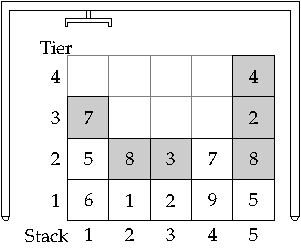
\includegraphics{figs/bay.pdf}
\caption{A container bay.}
\label{fig:bay}
\end{figure}

Each container is labeled with a group value $g \in[1,G]$. A container is \emph{orderly} if it is supported directly by the ground or another orderly container with equal or larger group value; otherwise, it is \emph{disorderly}. Other phrases which have the same meaning of ``orderly{\slash}disorderly'' in recent literature include ``well{\slash}badly placed''~\citep{bort2012}, ``well-{\slash}non-well-located''~\citep{exp2012}, and ``clean{\slash}dirty''~\citep{wang2015}.

Figure~\ref{fig:bay} gives an example of a bay with $S=5$, $H=4$, and $N=13$. Containers are represented by boxes with their group values marked inside. Boxes with gray backgrounds are disorderly containers.
The objective of the CPMP is to find an optimized sequence with the fewest container movements, by which all containers are rearranged to be orderly.
The movement sequence is called ``applied to'' the CPMP instance.




To better describe the solution to the CPMP, we represent layout-related items mathematically.
The tier and stack numbers of the bay are labeled from bottom to up and left to right, respectively.
Let $\mathbb{S}=\{1,\dots,S\}$ be the set of stacks. Hereafter, for simplification of description, when a stack $s$ is mentioned without declaring its domain, it is assumed that $s\in\mathbb{S}$. The height of stack $s$ is denoted by $h(s)$ and $e(s)=H-h(s)$ denotes the number of empty slots in $s$. Note that the height of stacks should not exceed $H$.
The orderly height (number of orderly containers) of $s$ is denoted by $o(s)$.

The slot positioned at $t$-th tier of stack $s$ is denoted by $(s,t)$.
The group value of a container $c$ is denoted by $g(c)$.
Likewise, the group value of a container located in slot $(s,t)$ is denoted by $g(s,t)$.







\section{State and state feasibility}
\label{sec:state}
\begin{definition}[Fixed containers]
A fixed container is an orderly container and not allowed to be moved in the following movement sequence.
\end{definition}
If a container is a fixed container, then the containers under it must be fixed containers.
\begin{definition}[State]
A state $(\mathsf{L},\boldsymbol{f})$ is a pair composed of a layout $\mathsf{L}$ and a fix vector $\boldsymbol{f}$.
\end{definition}
The {fix} vector $\boldsymbol{f}$ indicates the number of fixed containers (fixed height) in each stack of $\mathsf{L}$.
$f(s)$ is the $s$th element. Fixed and unfixed containers are separated by a line (a skyline), as shown in Figure~\ref{fig:skyline}.
In Figure \ref{fig:exp1}, $\boldsymbol f=(2,3,1)$; in Figure \ref{fig:exp2}, $\boldsymbol f=(2,3,0)$.

\begin{figure}[htbp]
\centering
\subfigure[]{
    \label{fig:exp1}
    \resizebox{0.35\textwidth}{!}{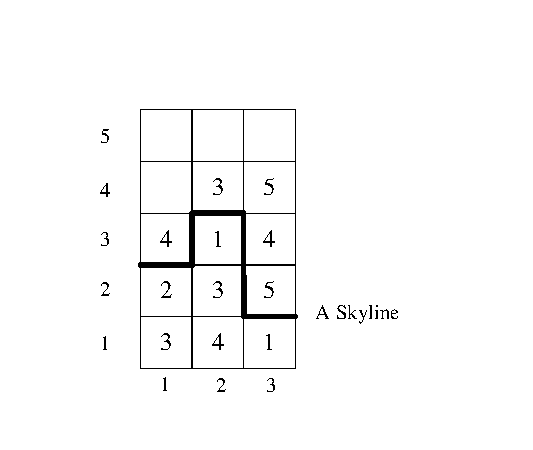
\includegraphics{figs/exp1.pdf}}}
\subfigure[]{
    \label{fig:exp2}
    \resizebox{0.35\textwidth}{!}{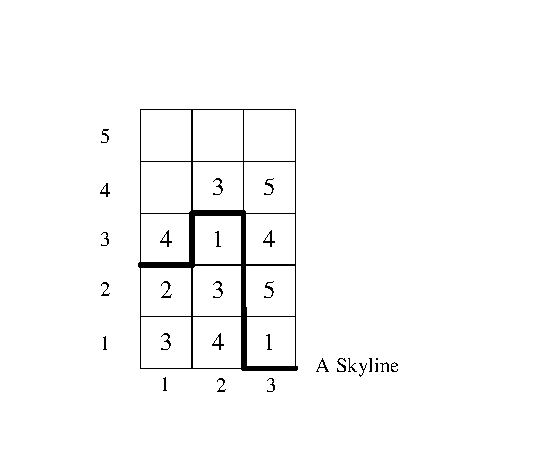
\includegraphics{figs/exp2.pdf}}}
\caption{Fix vector and skyline.}
\label{fig:skyline}
\end{figure}


It is noteworthy that if two states have the same layout but different fix vectors, then they are two different states, just like Figure~\ref{fig:exp1} and~\ref{fig:exp2}.

\begin{definition}[Feasibility of a state]
A state $(\mathsf{L},\boldsymbol{f})$ is feasible if there exists a movement sequence that can convert $\mathsf{L}$ to an orderly layout without moving fixed containers indicated by $f$.
\end{definition}

The necessary condition for state feasibility has been talked about in \citet{wang2014}. To make the content self-contained, we briefly explain it in this paper. Containers above the skyline can be moved, therefore slots and containers above the skyline now are separately considered.

For a stack $s$ in state $(\mathsf{L},\boldsymbol{f})$, suppose that the smallest group label under the skyline is $g$, then $H-f(s)$ slots are above the skyline and can only be placed with container $c$ satisfying $g(c)\le g$; otherwise, $s$ will be disorderly. In such a situation, we say stack $s$ has $H-f(s)$ slots with group label $g$.
If the skyline of $s$ coincides with the ground, then $s$ has $H$ slots with group label $G$.
For example, in Figure \ref{fig:exp2}, stack 1, 2 and 3 have 3, 2 and 5 slots with group label 2, 1 and 5, respectively. The total number of slots with group label $g$ in the whole bay is denoted by $r(g)$ (resource for group $g$).
Similarly, the number of unfixed containers with group label $g$ is denoted by $d(g)$ (demand of group $g$).
For a feasible state, the slots available for group $g$ must be more than the demand of group $g$. That is,
\begin{equation*}
\sum^G_{i=g+1}r(g)-\sum^G_{i=g+1}d(g)+r(g)\ge d(g)
\end{equation*}
which is equivalent to
\begin{equation*}
\sum^G_{i=g}r(g)\ge \sum^G_{i=g} d(g)
\end{equation*}

Denote $R(g)=\sum^G_{i=g}r(g)$ and $D(g)=\sum^G_{i=g}d(g)$. $\boldsymbol R$ and $\boldsymbol D$ are the two G-dimension vectors with elements $R(g)$ and $D(g)$, respectively. The above condition is expressed as $\boldsymbol{\Delta}=\boldsymbol{R}-\boldsymbol{D}\ge \boldsymbol{0}$. Here $\boldsymbol \Delta$ is called `surplus vector'.

\begin{proposition}[Necessary condition for state feasibility]
A necessary condition for a feasible state $(\mathsf{L},\boldsymbol{f})$ is $\boldsymbol{\Delta}=\boldsymbol{R}-\boldsymbol{D}\ge \boldsymbol{0}$.
\end{proposition}



Take the layouts in Figure~\ref{fig:exp1} and \ref{fig:exp2} as an example.
Table~\ref{tab:feasible} shows the surplus vectors for both cases. Case a is infeasible as only $\Delta(1)\ge0$; while the feasibility of Case b is not sure since $\boldsymbol \Delta\ge \boldsymbol {0}$ is a necessary condition. Intuitively, it can be seen that none of the three stacks in Figure~\ref{fig:exp1} can accommodate containers with group label 5 orderly, and this is the reason why Case a is infeasible.

\begin{table}[htbp]
\caption{Computation for the surplus vector.}
\centering

\begin{tabular}{c|c|c|c|c|c||c|c|c|c|c|c}
\hline
\multicolumn{6}{c||}{Case a} & \multicolumn{6}{c}{Case b}\\
\cline{1-6}
\cline{7-12}
$g$ & $d(g)$ & $D(g)$ & $r(g)$ & $R(g)$ & $\Delta(g)$ & $g$ & $d(g)$ & $D(g)$ & $r(g)$ & $R(g)$ & $\Delta(g)$\\
\hline
1   & 0      & 5      & 6      & 9      & 3           & 1   &  1     & 6       & 2      & 10     & 4\\
2   & 0      & 5      & 3      & 3      & -2          & 2   &  0     & 5       & 3      & 8      &  3\\
3   & 1      & 5      & 0      & 0      & -5          & 3   &  1     & 5       & 0      & 5      &  0\\
4   & 2      & 4      & 0      & 0      & -4          & 4   &  2     & 4       & 0      & 5      &  1\\
5   & 2      & 2      & 0      & 0      & -2          & 5   &  2     & 2       & 5      & 5      &  3\\
\hline
\end{tabular}
\label{tab:feasible}
\end{table}

The time complexity of checking $\boldsymbol{\Delta}\ge \boldsymbol{0}$ is only $\mathcal O(G)$.




\begin{definition}[Container stability]
Given a feasible state, a disorderly container is unstable. For any orderly container $c$ in slot $(s,t)$, try to fix container $c$ and those underneath it; if the resultant state has $\boldsymbol{\Delta}\ge 0$, then $c$ is stable. Otherwise, $c$ is unstable.
\end{definition}

According to the definition, an unstable container cannot be fixed in the current slot even if it is orderly, because the resultant state will be infeasible.
Unstable containers must be moved in the future. Denote the stable height (number of stable containers) of stack $s$ by $ \textit {sh}(s)$, then we have $\boldsymbol{f}\le \boldsymbol{sh}\le \boldsymbol{o}\le \boldsymbol{h}$. If a container $c$ is stable in stack $s$, we say that $s$ \emph{stabilizes} $c$.

Figure~\ref{fig:stable} gives an example of a state. Fixed containers are labeled with solid squares. Unstable containers are highlighted with gray backgrounds. Notice that the container $(2,1)$ with group value $6$ is orderly but unstable.

\begin{figure}[htbp]
\centering
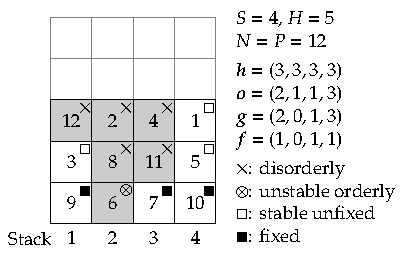
\includegraphics{figs/stable.pdf}
\caption{Stability of containers.}
\label{fig:stable}
\end{figure}

An orderly but unstable container indicates that its orderliness is valueless because it definitely requires at least one movement.
Using the concept of container stability instead of container orderliness is more precise in evaluating the layout.
For example, when selecting the placement of a blocking container, if the container is orderly but unstable after moving to a stack, then the attractiveness of such a movement should be reconsidered. The stability of containers should be recomputed after any container is fixed.

\begin{definition}[Extreme state]
A state $(\mathsf{L},\boldsymbol{f})$ is called an extreme state if $|\{s\in\mathbb{S}: f(s)=H\}|= S-2$.
\end{definition}

The definition of extreme state is to emphasize the especial case where $S-2$ stacks are fully fixed. In such a case, unfixed containers can only be moved between two stacks, say $a$ and $b$; the case is feasible if and only if one of the following conditions is satisfied:
\begin{enumerate}
\item Both stacks $a$ and $b$ are orderly;
\item Stack $a$ is orderly, and stack $b$ is disorderly. Disorderly containers in $b$ can be allocated to $a$ and $a$ is still orderly after the allocation.
\end{enumerate}

\begin{definition}[Dead-end state]
A state is called a dead-end state if it is an infeasible extreme state.
\end{definition}

The dead-end states are infeasible, therefore we should avoid generating them.
We have the following proposition:

\begin{proposition}[Existence of dead-end states]
No dead-end state can be generated whatever movements and fixed vectors are applied to instances with $E\ge2(H-1)$. For instances with $E<2(H-1)$, there exist possibilities of generating a dead-end state.
\end{proposition}
When $E\ge2(H-1)$, it has $N\le SH-2H+2$.
1) If there are fewer than S-2 stacks fully occupied, the state is not a dead-end state; 2) if there are S-2 stacks fully occupied, there are at most two extra containers in the left two stacks. The state is not a dead-end state, either. For cases with $E<2(H-1)$, there exist possibilities of generating a dead-end state.

As shown in Figure \ref{fig:non-dead-end}, it has $E\ge2(H-1)$, and it has no chance to generate dead-end states. In Figure~\ref{fig:dead-end} with $E<2(H-1)$, when $\boldsymbol f=(0,0,5,5)$, the state is a dead-end state.
\begin{figure}[htbp]
\centering
\subfigure[]{
    \label{fig:non-dead-end}
    \resizebox{0.2\textwidth}{!}{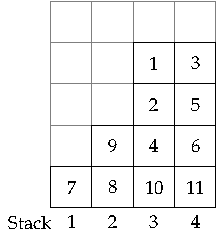
\includegraphics{figs/non-dead-end.pdf}}}
\subfigure[]{
    \label{fig:dead-end}
    \resizebox{0.2\textwidth}{!}{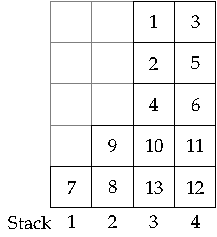
\includegraphics{figs/dead-end.pdf}}}
\caption{Existence of dead-end states.}
\end{figure}

\section{Feasibility-based heuristic}
\label{sec:fbh}

In this section, a feasibility-based heuristic (FBH) is developed for solving the CPMP\@. The proposed heuristic is a target-driven algorithm. Target-driven algorithms \citep{exp2012,wang2015} are efficient among all existing algorithms. Generally speaking, containers (targets) are rearranged to certain slots one by one, and each rearrangement is achieved by a sequence of movements. The heuristic can be implemented solely, then it is a greedy algorithm; the heuristic can also be the major component of other frameworks, such as GRASP and beam search.
In this work, we optimize the order of rearranging containers as well as the sequence of movements in one rearrangement.

The optimization is partially due to the concept of state feasibility. This is why our algorithm is called feasibility-based heuristic.
Before really rearranging a certain container, the feasibility of resultant state is checked. If the resultant state is infeasible, then we give up the rearrangement.
Due to the feasibility check, we can explore larger space without sacrificing efficiency: the order to rearrange containers is not fixed beforehand, but rather that it is decided as the algorithm goes on.






\subsection{Heuristic framework}
According to \citet{wang2014}, in dense instances with $E<H$, for a stack $s$, only the top $\sum_{i\neq s}e(i)$ containers can be moved to other stacks. The immovable number of containers (unreachable tiers) for any stack is $U=H-\sum_ie(i)=H-E$.
Containers in the bottom $H-E$ tiers of the bay are unreachable, that is, no sequence can move these containers.
In loose instances such that $E\ge H$, all containers in a stack are movable.
Let $U=\max\{H-E,0\}$ denotes the number of unreachable tiers for any instance.


The feasibility-based heuristic first constructs the initial state according to the unreachable tiers. In the initial state, $\mathsf L$ is the initial layout $\mathsf{L}^0$ and containers in unreachable tiers are fixed, i.e., $\boldsymbol f=U\cdot\boldsymbol{1}$, where $\boldsymbol 1$ is a S-dimension all-ones vector.

Starting from the initial state, the heuristic repeatedly fixes a target container $c^*$ to a target stack $s^*$.
Since $s^*$ has $f(s^*)$ fixed containers, $c^*$ is fixed at tier $f(s^*)+1$. The algorithm continues until all containers are fixed. The procedure of the heuristic is concisely described in Algorithm~\ref{algo:fbhs}.

\begin{algorithm}[htbp]
\caption{Feasibility-based heuristic.}
\label{algo:fbhs}


\setalgo


\Begin
{
  $(\mathsf{L},\boldsymbol{f})\gets (\mathsf{L}^0,U\cdot\boldsymbol{1})$\;
  \Repeat{$N-SU$}
  {
    $(c^*\rightarrow s^*)\gets\textrm{the selected valid task}$\;
    $\mathsf{L}$ = resultant layout after moving $c^*$ to $s^*$\;
    $f(s^*)\gets f(s^*)+1$\;
  }
}

\end{algorithm}

The procedure of selecting a task and moving $c^*$ to $s^*$ will be explained in Section~\ref{sec:task_sel} and ~\ref{sec:speedy}, respectively.

The advantage of fixing containers one by one lies in twofold: 1) movements are more target-oriented. Some works such as ~\cite{bort2012} move a container each time, but they don't have a clear aim. Hence, it is difficult to measure the benefit of movements and moreover, movements are blind: a container can be unnecessarily moved from stack $a$ to $b$ in a round and then moved from $b$ to $a$ after several rounds.
2) Fixed containers are not allowed to be moved, but unfixed orderly containers are allowed to be moved. This can distinguish fixed and unfixed orderly containers. Even though both are orderly, the statuses of both kinds are totally different. In works which does not distinguish fixed and unfixed containers, some containers do not need moved (fixed containers in our context), but they are involved in movements.


\subsection{Task selection}
\label{sec:task_sel}
\subsubsection{Valid task}
At every step of the heuristic, a {task} determines an unfixed container (target container) and a destination stack (target stack). Most target-driven algorithms select target containers according to a certain order, such as the descending order of group labels~\citep{exp2012}; in this research, the order to allocate containers is not fixed beforehand, but rather that it is decided as the algorithm goes on. This innovation undoubtedly enables the algorithm to search larger solution space, but the search efficiency may reduce. We use the feasibility to avoid useless solution space.
Our paper is the first work that uses feasibility to cut branches in CPMP algorithms.
A container--stack pair $c\rightarrow s$ is a valid task for the current state $( \mathsf{L},\boldsymbol{f})$ only if
\begin{itemize}
\item $c$ is unfixed,
\item $f(s)<H$,
\item $g(c)\le g(s,f(s))$, and
\item $\Delta(\varphi)\ge H-f(s), \varphi \in (g(c),g(s,f(s))]$.
\end{itemize}

The first condition is easy to understand. The second condition ensures that $s$ has a slot to accommodate $c$.
The third condition makes sure that the group label of $c$ is no larger than that of the highest fixed container of $s$.
The last condition ensures the non-negativity of the resultant surplus vector. If $c$ is moved to $s$, then the $g(c)$th element of demand vector $d[g(c)]$ decreases by 1, i.e., $d'[g(c)]=d[g(c)]-1$, while other elements do not change. In the meanwhile, for the resource vector, $r'[g(s,f(s))]=r[g(s,f(s))]-(H-f(s))$ while $r'[g(c)]=r[g(c)]+H-f(s)-1$, and other elements do not change. Then for $\varphi \in(g(c),g(s,f(s))]$, the feasible condition in the new layout is $D'(\varphi)=\sum_{g\ge \varphi}d'(g)=D(\varphi)\le R'(\varphi)=\sum_{g\ge\varphi}r'(g)=R(\varphi)-(H-f(s))$, i.e., $\Delta(\varphi)\ge H-f(s)$.

Pairs which satisfy the above conditions compose a set $\mathbb T$. However, the above conditions are only necessary conditions, so the feasibility of the resultant state is not sufficiently ensured, due to the possibility of dead-end states.

There are three methods for resolving the dead-end state issue.
\begin{enumerate}
\item Prevent from entering an extreme state when deciding the next task;
\item Design an ideal task accomplishment procedure that makes the resultant extreme state feasible;
\item Allow entering a dead-end state and relabel a fixed container as unfixed to run away from the dead-end state.
\end{enumerate}

Our previous work~\citep{wang2015} adopts the last method listed above. When the algorithm enters into a dead-end state, the algorithm relabels a fixed container as unfixed and moves it to a temporary slot; then the state becomes non-dead-end. After taking a sequence of movements, the relabeled container is recovered to its original slot. The disadvantage of such a choice is that running away from existing dead-end states costs many movements and these movements are unnecessary per se. A better choice is to avoid resulting in dead-end states when choosing valid tasks.

\begin{definition}[Pre-extreme state]
A feasible state is a pre-extreme state if $|\{s\in\mathbb{S}: f(s)=H\}|=S-3$, $|\{s\in\mathbb{S}: f(s)=H-1\}|\ge 1$ and $\sum_{s\in\mathbb{S}}f(s)<N-2$.
\end{definition}
The algorithm only explores states $(\mathsf{L},\boldsymbol{f})$ which satisfy $\boldsymbol{\Delta}\ge \boldsymbol{0}$.
When only three stacks have empty slots while the other $S-3$ stacks are fully fixed ($|s \in \mathbb S : f(s)= H| = S- 3$), and at least one stack has only one empty slot left $|s \in \mathbb S : f(s) = H-1| \ge 1$, let us investigate the validity of performing a task $c\rightarrow s$ with $f(s)=H-1$ based on the number of remaining unfixed containers.
\begin{enumerate}
\item If $\sum_{s\in\mathbb{S}} f(s) = N$, all the containers are fixed. The algorithm terminates with an orderly layout.

\item If $\sum_{s\in\mathbb{S}} f(s) = N-1$, only one container $c$ remains unfixed. As $\boldsymbol{\Delta}\ge \boldsymbol {0}$, and $D[g(c)]=d[g(c)]=1$, we have $S[g(c)]\ge1$, i.e., there is at least one slot which can accommodate $c$ orderly. At most one movement is needed to convert the layout to a feasible layout.

\item If $\sum_{s\in\mathbb{S}}f(s) = N-2$, two containers remain unfixed. Suppose the last two unfixed containers are $a$ and $b$, and the valid task is $a\rightarrow s$ with $f(s)=H-1$. When generating valid tasks, the fourth condition $\Delta(\varphi)\ge H-f(s), \varphi \in (g(c),g(s,f(s))]$ must be satisfied, i.e., the resultant layout $\mathsf L'$ after task $a\rightarrow s$ satisfies $\boldsymbol \Delta \ge \boldsymbol{0}$ and only $b$ is unfixed. Hence, $\mathsf L'$ can be converted into a feasible layout. Performing task $a\rightarrow s$ does not result in a dead-end state.

\item If $\sum f(s)_{s\in\mathbb{S}}\le N-3$, at least 3 containers remain unfixed. If the next task is to fix a container to a stack $s$ with $f(s)=H-1$, the resultant layout may be a dead-end state. Taking Figure~\ref{fig:pre-extreme} as an example. Containers with a solid square are fixed containers. For the task $1\rightarrow 3$, it is valid as the surplus vector of the resultant state is no less than zero. But the resultant state becomes dead-end.
\end{enumerate}

\begin{figure}[htbp]
\centering
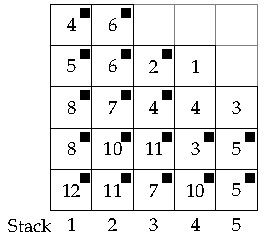
\includegraphics{figs/c.pdf}
\caption{Pre-extreme state.}
\label{fig:pre-extreme}
\end{figure}
Based on the above discussion, we can see that when $\sum_{s\in\mathbb{S}}f(s)<N-2$, there is a chance to generate dead-end state.

When the current state is a pre-extreme state, we eliminate the container--stack pairs $c\rightarrow s$ with $f(s)=H-1$ from $\mathbb T$, so that the algorithm avoids entering a dead-end state. This technique is called ``dead-end avoidance''
\subsubsection{Task evaluation}

Every valid task $c\rightarrow s\in\mathbb{T}$ is evaluated by a tuple with six elements: the tier-protection indicator, the number of moves required by the STAP, the number of stable containers that need to be moved from the aim stack $sh(s)-f(s)$, the affected demand, the fixed height of aim stack $f(s)$, and $-g(c)$.
The tuples of valid tasks are compared lexicographically, and the task with the minimum tuple is selected as the next task. The six elements in the tuple will be explained in the following.

The tier-protection indicator is to balance the trade-off between the freedom of task selection and the surplus loss. In principle, a container can be moved to any valid stack.
However, if a container with small group value occupies an (relatively) empty stack, then the loss of surplus vector is large: after the target container $c$ is fixed to the target slot $(s,f(s)+1)$, the surplus $\Delta(\varphi)$ is reduced by $H-f(s)$, for $\varphi\in (g(c),g(s,f(s))]$.
The larger the spread between $g(c)$ and $g(s,f(s))$ is, the more the surplus vector will lose. For example, in Figure \ref{fig:pre-extreme}, if container 1 positioned at (4,4) is moved on container 3 positioned at (5,3), the resource for group 3, namely $r(3)$ is reduced by 2 as 1 becomes the highest orderly container of stack 5. The cumulative resources $R(3)$ and $R(2)$ are reduced by 2 accordingly.

If a pair $c\rightarrow s$ satisfies $f(s)\le P1$ and affected demand $\sum_{\varphi=g(c)+1}^{g(s,f(s))}d(\varphi)\ge P2$, then the task is deleted from $\mathbb{T}$. As customizable parameters, the number of tiers protected $P1$ and the threshold value $P2$ can be adjusted optionally.

The number of moves required by the STAP is the number of movements needed for moving $c$ to $s$;
it is a precise number while in \citet{wang2015}, they just estimate the number of movements needed for moving $c$ to $s$.
The process to calculate the number is introduced in Section \ref{sec:speedy}.
The number of stable containers that need to be moved from the aim stack, namely, $\textit{sh}(s)-f(s)$ distinguishes stable and unstable orderly containers.
The affected demand is $\sum_{\varphi=g(c)+1}^{g(s,f(s))}d(\varphi)$.
The fixed height of aim stack favors low tiers, which makes the fixed height of stacks even.
The last element $-g(c)$ prefers large group values.


\subsection{Speedy task accomplishment procedure}

\label{sec:speedy}
After the task is decided, a speedy task accomplishment procedure (STAP) is carried out to accomplish the task, resulting in a new state. The movement sequence of STAP is based on task types.

Let the target container be denoted by $c^*$ (located in $(s^+,t^+)$) and the target stack by $s^*$. The task is \emph{immediate} if $c^*$ is just on the highest fixed container of $s^*$, i.e., $s^+=s^*$ and $t^+=f(s^*)+1$;
the task is \emph{internal} if $c^*$ is above but not immediately on the highest fixed container of $s^*$, i.e., $s^+=s^*$ and $t^+>f(s^*)+1$;
and the task is \emph{external} if $c^*$ and $s^*$ are in different stacks, i.e., $s^+\neq s^*$.


\subsubsection{Immediate task}

An immediate task does not require any move because the target container is already located in the target slot.

\subsubsection{Internal task}

For an internal task, let $a$ denote the number of empty slots except those in $s^+$ and one highest non-full stack; that is, $a=E-e(s^+)-\min_{s\neq s^+\&e(s)>0}e(s)$. If multiple stacks have the maximum height. Let $B_1$ ($b_1$) and $B_2$ ($b_2$) denote the set (numbers) of blocking containers above and below $c^*$ in $s^+$, respectively. Blocking containers refer to containers which are above a target container or a target slot.
The accomplishment procedure of an internal task is given in Algorithm~\ref{algo:internal}.

\begin{algorithm*}[htbp]

\caption{Accomplish an internal task.}
\label{algo:internal}

\setalgo

\SetKwProg{One}{case I1:}{}{end~case}
\SetKwProg{Two}{case I2:}{}{end~case}
\SetKwProg{Three}{case I3:}{}{end~case}
\SetKwInput{Target}{target container}
\SetKwInput{Aim}{aim slot}
\SetKwInput{Above}{blocking above}
\SetKwInput{Below}{blocking below}
\SetKwInput{Slot}{slot supply}

\begin{multicols}{2}
\Target{$c^*(s^+,t^+)$}

\Aim{$(s^+,f(s^+)+1)$}
\Slot{$a=E-e(s^+)-\min\{e(s):e(s)>0,s\neq s^+\}$}

\Above{$b_1=h(s^+)-t^+$}
\Below{$b_2=t^+-f(s^+)-1$}
  \One{$a\ge b_2$}
  {
    \Repeat{$b_1$}
    {
      $\mathbb{R}\gets \{s: s\neq s^+, h(s)<H,\, \alpha(s^+,s)\ge b_2\}$\;

      \Relocate{$s^+,1,\mathbb{R}$}\;
    }
    $\mathbb{I}\gets \{s:s\neq s^+: h(s)<H,\, E-e(s^+)-e(s)\ge b_2\}$\;

    $\mts\gets \Interim{$\mathbb{I}$}$\;
    \Move{$s^+,1,s'$}\;
    \Relocate{$s^+,b_2,\mathbb{S}\setminus\{s^+,\mts\}$}\;
    \Move{$\mts,1,s^+$}\;
    \tcp{I1:\ $h(s^+)-f(s^+)+1$ moves}
  }

  \Two{$a<b_2$ \& $|\{s\neq s^+: h(s)<H\}|>1$}
  {
    \Relocate{$s^+, b_1, \mathbb{S}\setminus\{s^+\}$}\;
    $\mts_1\gets \Interim{$\mathbb{S}\setminus\{s^+\}$}$\;
    \Move{$s^+, 1, \mts_1$}\;
    $k_2\gets E-e(s^+)-e(\mts_1)-1$\;
    \Relocate{$s^+, k_2, \mathbb{S}\setminus\{s^+,\mts_1\}$}\;
    Find $\mts_2$ s.t.\ $\mts_2\not\in \{s^+,\mts_1\}$ \& $h(\mts_2)<H$\;
    \Move{$\mts_1, 1, \mts_2$}\;
    \Move{$s^+, b_2-k_2, \mts_1$}\;
    \Move{$\mts_2, 1, s^+$}\;
    \tcp{I2:\ $h(s^+)-f(s^+)+2$ moves}
  }

  \Three{$a<b_2$ \& $|\{s\neq s^+: h(s)<H\}|=1$}
  {
    Find $s'$ s.t.\ $s'\neq s^+$ \& $h(s')<H$\;
    $\mts\gets \InterimFull{$\mathbb{S}\setminus\{s^+,s'\}$}$\;
    \BiSender{$\mts, 1, s^+, b_1, \{s'\}$}\;
    \Move{$s^+, 1, \mts$}\;
    \Move{$s^+, b_2, s'$}\;
    \Move{$\mts, 1, s^+$}\;
    \tcp{I3:\ $h(s^+)-f(s^+)+2$ moves}
  }

\end{multicols}
\BlankLine
\BlankLine
\end{algorithm*}

The accomplishment procedure is carried out based on the relationship between $a$ and $b_2$, which determines how containers are relocated.
\begin{itemize}
\item I1: $a\ge b_2$;
\item I2: $a<b_2$ \& $|\{s\neq s^+: h(s)<H\}|>1$;
\item I3: $a<b_2$ \& $|\{s\neq s^+: h(s)<H\}|=1$.
\end{itemize}

In case I1, $b_1$ containers above $c^*$ are relocated one by one. $\mathbb R$ represents the set of available destination stacks for the top container of $s^+$.
When relocating containers from $B_1$, reserving slots for containers from $B_2$ should be considered beforehand. Because $c^*$ is above $B_2$, so $c^*$ is relocated before containers of $B_2$.
If relocations put $c^*$ and $B_2$ in the same stack, then $c^*$ needs additional moves to be retrieved.

We reserve the stack with the minimum empty slots $s_{\text{min}}$ for $c^*$, and containers of $B_2$ can only be placed at stacks from set $\{s\in S: s\neq s^+, s\neq s_\text{min}\}$ ($a\ge b_2$).
When deciding whether a stack $s^{\text{dst}}$ can be the destination of a container $c$ from $B_1$, $\alpha$ function is used to compute if $c$ is placed to $s^{\text{dst}}$ how many slots left for $B_2$.
If the left slots are not enough for $B_2$, $c$ cannot be moved to $s^{\text{dst}}$.
$\alpha$ function is presented in Algorithm \ref{algo:alpha}.
\begin{algorithm}[htbp]

\caption{Alpha function.}
\label{algo:alpha}
\setalgo
\begin{multicols}{2}
\Function{$\alpha(s^+,\mds)$}
        {\tcp{$s^+\neq \mds$}
            $e^{\min}\gets \min\{e(s)>0:s\neq s^+\}$\;
            $e^{\sec}\gets \min\{e(s)>e^{\min}:s\neq s^+\}$\;
            $k^{\min}\gets |\{s\neq s^+ : e(s)=e^{\min}\}|$\;
            \uIf{$e(\mds)> e^{\min}$}
            {
                \Return $E-e(s^+)-e^{\min}-1$\;
            }
            \uElseIf{$e^{\min}\ge 2$}
            {
                \Return $E-e(s^+)-e^{\min}$\;
            }
            \uElseIf{$k^{\min}=1$}
            {
                \Return $E-e(s^+)-e^{\sec}-1$\;
            }
            \Else
            {
                \Return $E-e(s^+)-2$\;
            }
        }
\end{multicols}
\BlankLine
\BlankLine
\end{algorithm}

If $e(\mds)> e^{\min}$, that is, $\mds$ is not the highest non-full stack, $e^{\min}$ is reserved for $c^*$.
If $c$ is moved to $\mds$, left slots for $B_2$ is $E-e(s^+)-e^{\min}-1$.

If $e(\mds)=e^{\min}\ge 2$, that is, $\mds$ is the highest non-full stack and it has at least 2 empty slots. If $c$ is moved to $\mds$, the stack can also accommodate $c^*$, hence, left slots for $B_2$ is $E-e(s^+)-e^{\min}$.

If $e(\mds)=e^{\min}=1$ and $k^{\min}=1$, that is, $\mds$ is the unique highest stack with only one empty slot. If $c$ is moved to $\mds$, the stack with the second highest height will be reserved for $c^*$ in the next round. The number of slots left for $B_2$ becomes $E-e(s^+)-e^{\text{sec}}-1$.

If $e(\mds)=e^{\min}=1$ and $k^{\min}\ge2$, at least one stack with only one empty slot can accommodate $c^*$ in the future. If $c$ is moved to $\mds$, the number of slots left for $B_2$ becomes $E-e(s^+)-2$.

Function \Relocate{$\mss,k,\mathbb{R}$} is illustrated in Algorithm~\ref{algo:relocation}, which relocates $k$ containers from a {sender} stack $\mss$ to $\mathbb R$. For each of the top $k$ containers of the sender, the destination stack $\mds$ is properly selected from $\mathbb{R}$ according to the evaluation by function \EvalMove{$\mss,\mds$}. Function \Move{$\mss,k,\mds$} moves $k$ containers from $\mss$ to $\mds$.


\begin{algorithm}[htbp]

\caption{Relocate containers.}
\label{algo:relocation}
\setalgo
\begin{multicols}{2}


\Function{\Relocate{$\mss,k,\mathbb{R}$}}
{
  \Repeat{k}
  {
    $\mathbb{R}'\gets \{s\in \mathbb{R}:h(s)<H\}$\;
    $\mds\gets \arg\min_{s\in\mathbb{R}'} \EvalMove{$\mss,s$}$\;
    \Move{$\mss,1,\mds$}\;
  }
}

\end{multicols}
\BlankLine
\BlankLine
\end{algorithm}
\EvalMove{$\mss,\mds$} returns a tuple, the first element indicates the type of the penalty and the second element indicates the scale of the penalty of moving from $\mss$ to $\mds$ (refer to Algorithm~\ref{algo:eval_move}).
\begin{algorithm}[htbp]

\caption{Evaluate movements.}
\label{algo:eval_move}
\setalgo
\begin{multicols}{2}
\Function{\EvalMove{$\mss,\mds$}}
{
  $c\gets (\mss,h(\mss))$\;
  $g\gets g(c)$\;
  $q\gets q(\mds,h(\mds))$\;
  \uCase{$ sh(\mds)=h(\mds)$ \& stack $\mds$ can stabilize $c$}
  {
    \Return $\langle1, \sum_{\varphi=g+1}^q d(\varphi)\rangle$\;
  }
  \uCase{$ sh(\mds)<h(\mds)$ \& $g\ge m(\mds)$}
  {
    \Return $\langle2,g-m(\mds)\rangle $\;
  }
  \uCase{$ g(\mds)<h(\mds)$ \& $g<m(\mds)$}
  {
    \Return $\langle3, m(\mds)-g \rangle$\;
  }
  \Case{$ g(\mds)=h(\mds)$ \& stack $s_2$ cannot stabilize $c$}
  {
    \Return $\langle 4,q \rangle$\;
  }
}
\end{multicols}
\BlankLine
\BlankLine
\end{algorithm}


Let us define the capability of an occupied slot $(s,t)$ by $q(s,t) = g(s, t)$ if the container inside is orderly, otherwise $q(s, t) = 0$; specifically, the ground is regarded as an occupied slot at tier 0 with group value G.
Define the \emph{messiness} of stack $s$ by $m(s)=\max_{sh(s)<t\le h(s)}g(s,t)$, that is, the largest group value among the unstable containers in $s$.

As $\mds\gets \arg\min_{s\in\mathbb{R}'} \EvalMove{$\mss,s$}$, the preference of selecting $\mds$ for a blocking container $c$ is as follows:
\begin{enumerate}
\item If stack $\mds$ is entirely stable and can stabilize $c$, the stack with the minimum affected demand is preferred;
\item If stack $\mds$ is not entirely stable and $g(c)\ge m(\mds)$, the stack with the minimum gap between $m(\mds)$ and $g(c)$ is preferred;
\item If stack $\mds$ is not entirely stable and $g(c)> m(\mds)$, the stack with the minimum gap between $g(c)$ and $m(\mds)$ is preferred;
\item If stack $\mds$ is entirely stable but cannot stabilize $c$, the stack with the minimum $q(\mds,h(\mds))$ is preferred.
\end{enumerate}

The first preference indicates that stabilizing a blocking container reduces the total number of unstable containers in the bay. The second and third preferences consider the messiness of the destination stack.
Larger messiness implies a higher urgency of reshuffles. The last preference indicates that an entirely stable stack should be protected from being ruined.



In cases I1 and I2, an interim stack is selected to temporarily store the target container (function \Interim{$\mathbb{I}$}).
The selection prefers stacks that are not entirely stable with the largest messiness, then entirely stable stacks with the smallest group value of orderly containers.
The most unattractive stack for receiving blocking containers is selected as the interim stack. In cases I3 and E4 (in Section~\ref{sec:external}), the interim stack is selected by the minimum group value of the top containers of full stacks, which is function \InterimFull{$\mathbb{F}$}.

\begin{algorithm}[htbp]

\caption{Interim and InterimFull functions.}

\setalgo
\begin{multicols}{2}
\Function{\Interim{$\mathbb{I}$}}
{
  $\mathbb{I}_1\gets \{s\in \mathbb{I}:  sh(s)<h(s)<H\}$\;
  $\mathbb{I}_2\gets \{s\in \mathbb{I}:  sh(s)=h(s)<H\}$\;

  \uIf{$\mathbb{I}_1\neq \varnothing$}
  {
    \Return $\arg\max_{s\in\mathbb{I}_1} m(s)$\;
  }
  \Else
  {
    \Return $\arg\min_{s\in\mathbb{I}_2} q(s,h(s))$\;
  }

}




\Function{\InterimFull{$\mathbb{F}$}}
{
  $\mathbb{F}_1\gets \{s\in \mathbb{F}: f(s)\le sh(s)<h(s)=H\}$\;
  $\mathbb{F}_2\gets \{s\in \mathbb{F}: f(s)< sh(s)=h(s)=H\}$\;
  \uIf{$\mathbb{F}_1\neq \varnothing$}
  {
    \Return $\arg\min_{s\in\mathbb{F}_1} g(s,h(s))$\;
  }
  \Else
  {
    \Return $\arg\min_{s\in\mathbb{F}_2} g(s,h(s))$\;
  }
}

\end{multicols}
\BlankLine
\BlankLine
\end{algorithm}

Function \BiSender{$\mss_1,k_1,\mss_2,k_2,\mathbb{R}$} performs relocations from two senders $\mss_1$ and $\mss_2$ to a receiver set $\mathbb{R}$, and the respective relocation quantities are $k_1$ and $k_2$.
The two top containers from two senders is compared and the one with a smaller tuple is moved first. In Algorithm~\ref{algo:bisender}, $\vec{v}_1$ and $\vec{v}_2$ are tuple results of function \EvalMove.

Likewise, function \BiReceiver{$\mss,k_1,\mathbb{R}_1,k_2,\mathbb{R}_2$} in the external case relocates $k_1$ and $k_2$ containers from one sender $\mss$ to two receiver sets $\mathbb{R}_1$ and $\mathbb{R}_2$, respectively.

\begin{algorithm}[htbp]

\caption{BiSender and BiReceiver functions.}
\label{algo:bisender}
\setalgo


\begin{multicols}{2}
\Function{\BiSender{$\mss_1,k_1,\mss_2,k_2,\mathbb{R}$}}
{
  $i\gets k_1$, $j\gets k_2$\;
  \Repeat{$k_1+k_2$}
  {
    \uIf{$j=0$}{
      \Relocate{$\mss_1,i,\mathbb{R}$}\;
      $i\gets 0$\;
    }
    \uElseIf{$i=0$}{
      \Relocate{$\mss_2,j,\mathbb{R}$}\;
      $j\gets 0$\;
    }
    \Else
    {
      $\mathbb{R}'\gets \{s\in \mathbb{R}:h(s)<H\}$\;
      $\mds_1\gets \arg\min_{s\in\mathbb{R}'} \EvalMove{$\mss_1,s$}$\;
      $\vec{v}_1\gets \EvalMove{$\mss_1,\mds_1$}$\;
      $\mds_2\gets \arg\min_{s\in\mathbb{R}'} \EvalMove{$\mss_2,s$}$\;
      $\vec{v}_2\gets \EvalMove{$\mss_2,\mds_2$}$\;
      \eIf{$\vec{v}_1\le^{\mathrm{lex}} \vec{v}_2$}
      {
        \Move{$\mss_1,1,\mds_1$}\;
        $i\gets i-1$;
      }
      {
        \Move{$\mss_2,1,\mds_2$}\;
        $j\gets j-1$\;
      }
    }
  }
}

\Function{\BiReceiver{$\mss,k_1,\mathbb{R}_1,k_2,\mathbb{R}_2$}}
{
  $i\gets k_1$, $j\gets k_2$\;
  \Repeat{$k_1+k_2$}
  {
    \uIf{$j=0$}{
      \Relocate{$\mss,i,\mathbb{R}_1$}\;
      $i\gets 0$\;
    }
    \uElseIf{$i=0$}
    {
      \Relocate{$\mss,j,\mathbb{R}_2$}\;
      $j\gets 0$\;
    }
    \Else
    {
      $\mathbb{R}_1'\gets \{s\in \mathbb{R}_1:h(s)<H\}$\;
      $\mathbb{R}_2'\gets \{s\in \mathbb{R}_2:h(s)<H\}$\;


      $\mds_1\gets \arg\min_{s\in\mathbb{R}_1'} \EvalMove{$\mss,s$}$\;
      $\vec{v}_1\gets \EvalMove{$\mss,\mds_1$}$\;
      $\mds_2\gets \arg\min_{s\in\mathbb{R}_2'} \EvalMove{$\mss,s$}$\;
      $\vec{v}_2\gets \EvalMove{$\mss,\mds_2$}$\;

      \eIf{$\vec{v}_1\le^{\mathrm{lex}}\vec{v}_2$}
      {
        \Move{$\mss,1,\mds_1$}\;
        $i\gets i-1$\;
      }
      {
        \Move{$\mss,1,\mds_2$}\;
        $j\gets j-1$\;
      }
    }
  }
}

\end{multicols}

\BlankLine
\BlankLine
\end{algorithm}

The total number of moves needed in case I1 is $h(s^+)-f(s+)+1$, and the numbers of moves in case I2 and case I3 are $h(s^+)-f(s+)+2$. All are noted in the comments of Algorithm~\ref{algo:internal}.

Note that in case I2, the target container $c^*$ is moved to the new interim stack $\mts_2$ from the first interim stack $\mts_1$ when there is only one empty slot in $\mathbb{S}\setminus\{s^+,\mts_1\}$.
This can be modified so that $c^*$ can be moved to a new interim stack $\mts_2$ earlier as long as the empty slots in $\mathbb{S}\setminus\{s^+,\mts_2\}$ are enough for containers in $B_2$. Moreover, if there is a full stack in $\mathbb{S}\setminus\{s^+\}$ in case I2, the task can also be completed in a similar way as that used in case I3 with the same operational cost.

\subsubsection{External task}
\label{sec:external}
For an external task, the number of empty slots in $\mathbb{S}\setminus\{s^+,s^*\}$ is denoted by $a$; that is, $a=E-e(s^+)-e(s^*)$. Let $B_1$ $(b_1)$ and $B_2$ $(b_2)$ denote the set (numbers) of blocking containers above the target container $c^*$ and the aim slot $(s^*,f(s^*))$, respectively. The pseudo-code describing the accomplishment for an external task is given in Algorithm~\ref{algo:external}. Four situations are considered.
\begin{itemize}
\item E1: $a\ge b_1+b_2$;
\item E2: $b_1+1\le a<b_1+b_2$;
\item E3: $1\le a<b_1+\min\{1,b_2\}$;
\item E4: $a=0<b_1+b_2$.
\end{itemize}



\begin{algorithm*}[htbp]
\caption{Accomplish an external task.}
\label{algo:external}

\setalgo

\SetKwProg{One}{case E1:}{}{end~case}
\SetKwProg{Two}{case E2:}{}{end~case}
\SetKwProg{Three}{case E3:}{}{end~case}
\SetKwProg{Four}{case E4:}{}{end~case}
\SetKwInput{Target}{target container}
\SetKwInput{Aim}{aim slot}
\SetKwInput{BPlus}{blocking above target}
\SetKwInput{BMinus}{blocking in aim stack}
\SetKwInput{Slot}{slot supply}


\begin{multicols}{2}

\Target{$c^*(s^+,t^+)$}
\Aim{$(s^*,f(s^*)+1)$}
\BPlus{$b_1=h(s^+)-t^+$}
\BMinus{$b_2=h(s^*)-f(s^*)$}
\Slot{$a=E-e(s^+)-e(s^*)$}

  \One{$a\ge b_1+b_2$}
  {
    \BiSender{$s^+, b_1,s^*,b_2, \mathbb{S}\setminus\{s^+,s^*\}$}\;
    \Move{$s^+, 1, s^*$}\;
    \tcp{E1:\ $b_1+b_2+1$ moves}
  }

  \Two{$b_1+1\le a<b_1+b_2$}
  {
    $k_2\gets a-1-b_1$\;
    \BiSender{$s^+, b_1, s^*, k_2, \mathbb{S}\setminus\{s^+,s^*\}$}\;
    Find $\mts$ s.t.\ $\mts\not\in \{s^+,s^*\}$ \& $h(\mts)<H$\;
    \Move{$s^+,1,\mts$}\;
    \Move{$s^-, b_2-k_2, s^+$}\;
    \Move{$\mts, 1, s^*$}\;
    \tcp{E2:\ $b_1+b_2+2$ moves}
  }


  \Three{$1\le a<b_1+\min\{1,b_2\}$}
  {
    $k_1\gets a-1$\;
    \BiReceiver{$s^+, k_1, \mathbb{S}\setminus\{s^+,s^*\}, b_1-k_1, \{s^*\}$}\;
    Find $\mts$ s.t.\ $\mts\not\in \{s^+,s^*\}$ \& $h(\mts)<H$\;
    \Move{$s^+,1,\mts$}\;
    \Move{$s^*, b_1-k_1+b_2, s^+$}\;
    \Move{$\mts, 1, s^*$}\;
    \tcp{E3:\ $2b_1+b_2-a+3$ moves}
  }

  \Four{$a=0<b_1+b_2$}
  {
    $\mts\gets \InterimFull{$\mathbb{S}\setminus\{s^+,s^*\}$}$\;
    \BiSender{$\mts, 1, s^+, b_1, \{s^*\}$}\;
    \Move{$s^+, 1, \mts$}\;
    \Move{$s^*, b_1+b_2+1, s^+$}\;
    \Move{$\mts, 1, s^*$}\;
    \tcp{E4:\ $2b_1+b_2+4$ moves}
  }

\end{multicols}

\BlankLine
\BlankLine
\end{algorithm*}

\section{Computational results}
\label{sec:experiment}

In this section, the proposed feasibility-based heuristic (FBH) is compared to four benchmark approaches; three methods are heuristics: the target-guided heuristic (TGH) proposed in our previous work \citep{wang2015}, an implementation of the LPFH proposed by \citet{exp2012}, and an implementation of the multi-heuristic proposed by \citet{jovanovic2014}. The fourth method BS-B is a beam search framework consolidating TGH as a component \citep{wang2015}. By far, BS-B has the best performance. It is necessary to estimate the quality level of FBH with the best known values.
The constructive heuristic can be embedded later into a frame such as beam search and GRASP to improve the solution quality.

Both LPFH and multi-heuristic approach do not report results on BF data set. Thus, we implemented LPFH and multi-heuristic approach by ourselves.
The original LPFH involves with randomness, we developed a deterministic one instead, referred to as the largest group value first heuristic~(LGVFH). The LGVFH selects the next target container from unfixed containers with the largest group value, and then accomplish it by the STAP\@. The pseudo-code for the LGVFH is given in Algorithm~\ref{algo:lpvfh}.

\begin{algorithm*}[htbp]
\caption{Largest group value first heuristic.}
\label{algo:lpvfh}


\setalgo

\begin{multicols}{2}

\Begin
{
  $(\mathsf{L},\boldsymbol{f})\gets (\mathsf{L}^0,U\cdot\boldsymbol{1})$\;

  \ForEach{$g=G,\dots,1$}
  {
    $\mathbb{C}_g\gets\textrm{containers with group value $g$}$\;
    $\mathbb{A}_g\gets\varnothing$\tcp*[l]{set of aim stacks}
    \While{$\mathbb{C}_g\neq \varnothing$}
    {
      $(c^*, s^*)\gets \arg\min_{c\in\mathbb{C}_g, f(s)<H} \MoveNeed{$c,s$}$\;
      Accomplish $( c^*, s^-)$ by the STAP\;
      $f(s^*)\gets f(s^*)+1$\;
      $\mathbb{C}_g\gets\mathbb{C}_g\setminus\{c^*\}$\;
      $\mathbb{A}_g\gets \mathbb{A}_g\cup \{s^*\}$\;
    }
    \ForEach{$s^*\in\mathbb{A}_g$}
    {
    	\Fill{$s^*$}\;
    }
  }
}



\Function{\Fill{$s$}}
{
  \While{$h(s)<H$}
  {
    $\mathbb{S}'\gets\varnothing$\;
    \ForEach{$i\in\{i\neq s: sh(i)<h(i)\}$}
    {
      $c\gets (i,h(i))$\;
      \If{ stack $s$ can stabilize $c$}
      {
        $\mathbb{S}'\gets \mathbb{S}'\cup \{i\}$\;
      }
    }
    \eIf{$\mathbb{S}'\neq \varnothing$}
    {
      $s'\gets \arg\max_{i\in\mathbb{S}'} g(i,h(i))$\;
      \Move{$s',1,s$}\;
    }
    {
      \Break\;
    }
  }
}
\end{multicols}
\BlankLine
\BlankLine
\end{algorithm*}

Here, function \MoveNeed{$c,s$} is the actual number of moves needed by the STAP to accomplish the task $(c,s)$. Function \Fill{$s$} is achieved by fulfilling $s$ with unstable containers in other stacks which $s$ can stabilize.

Experiments were conducted on a PC with Intel Core i7 CPU clocked at 3.40~GHz with Windows 7 operating system. The code was written in Java.

\subsection{Configuration of P1 and P2}
This section shows the effect of the tier-protection indicator. We selected six settings of the two parameters $(P1,P2$), which is $(0,N), (H/4,N/2), (H/3,N/6), (2H/3,N/8), (H,N/10)$. We made $P1$ and $P2$ proportional to $H$ and $N$, respectively, since $f(s)$  and the affected demand are related to the height and number of containers, respectively.

The six settings are in a loose-intermediate-tight order, and algorithms will filter out more tasks when using back settings. The result is shown in Table~\ref{tab:tier-protection}.
The first column indicates the parameter setting. The second and third columns indicate the average movements of CVS and BF data sets, respectively.
Parameter $(0,N)$ means that there is no tier-protection indicator so no task is filtered out. As the setting becomes tight, the performance of both CVS and BF is improved, until a peak is achieved. But when the setting becomes extremely tight, the performance decreases. When the setting is $(H,N/10)$, some instances of CVS even cannot find a solution; therefore, we mark the unit with ``Nil''. The instances of BF are loose, that is, the empty slots are sufficient. Solutions can be found even if under setting $(H,N/10)$, but the performance is worse than that with an intermediate setting.
\begin{table}[htbp]
  \centering
  \caption{Configuration of $P1$ and $P2$.}
    \begin{tabular}{lrr}
    \toprule
    $(P1,P2)$ & CVS   & BF \\
    \midrule
    $(0,N)$   & 52.15 & 71.69 \\
    $(H/4,N/2)$ & 50.43 & 71.21 \\
    $(H/3,N/4)$ & 45.82 & 69.05 \\
    $(H/2,N/6)$ & 45.32 & 69.51 \\
    $(2H/3,N/8)$ & 46.33 & 71.23 \\
    $(H,N/10)$ & Nil   & 73.44 \\
    \bottomrule
    \end{tabular}
  \label{tab:tier-protection}
\end{table}



\subsection{Results for CVS instances}

\citet{cas2011} present the complete CVS data set (named after the authors' surnames, Caserta, Vo{\ss} and Sniedovich) originally for the CRP\@. The CVS instances are classified into 21 groups, each consisting of 40 instances.
The heights of piled containers in each stack are the same, denoted by $K$, hence $N=SK$. It is worth noting that the height limitation of each stack is not specified in the original data.
Researchers add two extra tiers above the initial layout in order to make the data suit for the CPMP problem; that is, $H=K+2$.

The CVS instances can be considered as typical dense CPMP instances.
Table~\ref{tab:cvs} illustrates the computational results on CVS instances by the TGH, the LGVFH, the multi-heuristic approach, the FBH, and the BS-B\@.
The column ``Opt'' is the optimal values achieved by A*.
The values under the ``moves'' headings represent average numbers of moves for every CVS group, whereas the values under the ``time (ms)'' headings are the run time in ms. The values under the ``improvement'' heading are the improvements compared to TGH, LGVFH, and multi-heuristic in percentage.
The results showcase that the FBH surpasses the TGH and LGVFH by more than $10\%\times N$ moves on most instance groups. Especially on the narrowest group CVS~10-6, the FBH outperforms the TGH and LGVFH by 319.38\% and 55.54\%, respectively. For the comparison to the multi-heuristic approach, the FBH is better for some instances while the multi-heuristic is better for other instances.
\begin{landscape}
\begin{table}[htbp]
\caption{Results for CVS instances.}
\label{tab:cvs}

\settab

\centering
\begin{tabular}{ccccccccccccccc}
\toprule
\multirow{2}{*}{CVS~K-S}&

\multicolumn{2}{@{}c@{}}{TGH}
&
\multicolumn{2}{@{}c@{}}{LGVFH}
&
\multicolumn{2}{@{}c@{}}{multi}
&
\multicolumn{2}{@{}c@{}}{FBH}
&
\multicolumn{2}{@{}c@{}}{BS-B}
&
Opt
&
\multicolumn{3}{@{}c@{}}{improvement}\\

\cmidrule(r){2-12}
\cmidrule{13-15}
          & moves&time (ms)&moves  &time (ms)& moves&  time (ms) &moves & time (ms)& moves  & time (ms) & moves & TGH & LGVFH & multi\\
\midrule
CVS 3-3   & 12.95  & 0.43 & 11.25  & 0.45 & 10.23  & 0.50 & 11.28  & 0.53  & 9.35  & 7.05    & 8.78 &12.93\%   & $-$0.22\%  & $-$10.27\%\\
CVS 3-4   & 12.18  & 0.20 & 12.23  & 0.15 & 10.98  & 0.50 & 10.80  & 0.18  & 9.45  & 7.83    & 9.03 & 11.29\%  & 11.66\%  & 1.59\%\\
CVS 3-5   & 12.78  & 0.10 & 13.45  & 0.20 & 12.23  & 0.75 & 12.08  & 0.18  & 10.45 & 12.55   & 10.15& 5.48\%   & 10.22\%  & 1.23\%\\
CVS 3-6   & 14.38  & 0.18 & 14.88  & 0.33 & 13.98  & 0.50 & 12.98  & 0.23  & 11.58 & 19.18   & 11.28& 9.74\%   & 12.77\%  & 7.16\%\\
CVS 3-7   & 16.00  & 0.13 & 16.58  & 0.23 & 15.83  & 0.50 & 14.75  & 0.15  & 13.13 & 31.63   & 12.80& 7.81\%   & 11.01\%  & 6.79\%\\
CVS 3-8   & 16.55  & 0.15 & 17.08  & 0.28 & 16.93  & 1.25 & 15.65  & 0.38  & 13.90 & 46.88   & 13.68& 5.44\%   & 8.35\%   & 7.53\%\\
CVS 4-4   & 23.35  & 0.05 & 21.93  & 0.08 & 20.38  & 1.53 & 21.88  & 0.15  & 16.98 & 61.35   & 15.83& 6.32\%   & 0.23\%   & $-$7.36\%\\
CVS 4-5   & 26.73  & 0.10 & 26.48  & 0.18 & 23.78  & 0.75 & 23.08  & 0.18  & 18.90 & 112.08  & 21.05& 13.66\%  & 12.84\%  & 2.94\%\\
CVS 4-6   & 27.58  & 0.08 & 27.20  & 0.23 & 25.90  & 0.75 & 24.75  & 0.48  & 20.25 & 191.50  & -    & 10.24\%  & 9.01\%   & 4.44\%\\
CVS 4-7   & 29.93  & 0.08 & 31.23  & 0.38 & 29.63  & 0.75 & 27.63  & 0.10  & 23.15 & 331.18  & -    & 7.69\%   & 11.53\%  & 6.75\%\\
CVS 5-4   & 44.83  & 0.08 & 35.83  & 0.18 & 31.78  & 2.25 & 35.08  & 0.08  & 26.43 & 221.13  & -    & 21.75\%  & 2.09\%   & $-$10.39\%\\
CVS 5-5   & 42.40  & 0.05 & 36.50  & 0.25 & 33.63  & 2.50 & 35.33  & 0.23  & 27.38 & 394.60  & -    & 16.69\%  & 3.22\%   & $-$5.06\%\\
CVS 5-6   & 50.63  & 0.13 & 43.08  & 0.23 & 40.73  & 2.75 & 39.88  & 0.23  & 32.08 & 996.90  & -    & 21.24\%  & 7.43\%   & 2.09\% \\
CVS 5-7   & 48.83  & 0.13 & 46.95  & 0.73 & 44.35  & 3.50 & 41.68  & 0.28  & 34.20 & 1507.13 & -    & 14.64\%  & 11.24\%  & 6.03\%\\
CVS 5-8   & 56.68  & 0.20 & 51.83  & 0.63 & 50.48  & 6.00 & 47.50  & 0.48  & 38.63 & 3030.35 & -    & 16.19\%  & 8.35\%   & 5.89\%\\
CVS 5-9   & 57.50  & 0.08 & 55.65  & 1.08 & 55.28  & 7.00 & 50.45  & 0.90  & 42.15 & 4615.30 & -    & 12.26\%  & 9.34\%   & 8.73\%\\
CVS 5-10  & 62.80  & 0.53 & 60.88  & 1.30 & 59.6   & 7.00 & 54.63  & 0.80  & 44.85 & 7455.93 & -    & 13.02\%  & 10.27\%  & 8.35\%\\
CVS 6-6   & 74.33  & 0.13 & 57.85  & 0.28 & 54.00  & 4.25 & 55.23  & 0.50  & 43.80 & 2511.33 & -    & 25.70\%   & 4.54\%   & $-$2.27\%\\
CVS 6-10  & 88.63  & 0.43 & 79.73  & 1.88 & 79.58  & 14.75& 75.60  & 1.65  & 60.55 & 23423.80 & -    & 14.70\%   & 5.17\%   & 5.00\%\\
CVS 10-6  & 332.25 & 0.30 & 173.95 & 1.08 & 150.28 & 18.28& 140.63 & 0.85 & 116.18 & 23010.70 & -    & 57.57\%  & 19.16\%  & 6.42\%\\
CVS 10-10 & 302.90 & 0.90 & 190.50 & 5.05 & 181.58 & 59.78&179.23  & 3.65  & 150.18 & 287920.50 & -  & 40.83\%  & 5.92\%   & 1.29\%\\[\defaultaddspace]
Average   & 64.48  & 0.21 & 48.81  & 0.72 & 45.77  & 6.47 &44.29  & 0.58  & 36.36 & 16948.04 & -    & 16.44\%  & 8.29\%   & 2.23\%\\
\bottomrule
\end{tabular}
\end{table}
\end{landscape}
\subsection{Results for BF instances}

\citet{bort2012} introduce 32 groups of CPMP instances (referred to as BF instances); each group consists of 20 instances. In BF instances, the bay size is $S=16$ or $20$ and $H=5$ or $8$. The number of containers $N$ is either $0.6\times SH$ or $0.8\times SH$, the number of groups $G$ is either $0.2\times N$ or $0.4\times N$, and the number of disorderly containers $B$ is either $0.6\times N$ or $0.75\times N$ in the initial layout.

The BF instances can be considered as typical loose CPMP instances. Table~\ref{tab:bf} illustrates the computational results on BF instances by the five methods. The values under the ``moves'' headings represent average numbers of moves for every BF group solved by different algorithms, whereas the values under the ``time (ms)'' headings are the run time in ms. The values under the ``improvement'' heading are the improvements compared to TGH, LGVFH and multi-heuristic approach in percentage.
\begin{landscape}
\begin{table}[htbp]
\caption{Results for BF instances.}
\label{tab:bf}

\settab

\centering

\begin{tabular}{ccccccccccccccccccc}
\toprule
\multirow{2}{*}[-.5\defaultaddspace]{BF} &
\multirow{2}{*}[-.5\defaultaddspace]{S}   &
\multirow{2}{*}[-.5\defaultaddspace]{H}    &
\multirow{2}{*}[-.5\defaultaddspace]{N}   &
\multirow{2}{*}[-.5\defaultaddspace]{G}    &
\multirow{2}{*}[-.5\defaultaddspace]{B}   &
\multicolumn{2}{@{}c@{}}{TGH} & \multicolumn{2}{@{}c@{}}{LGVFH} & \multicolumn{2}{@{}c@{}}{multi} & \multicolumn{2}{@{}c}{FBH} & \multicolumn{2}{@{}c}{BS-B} &
\multicolumn{3}{@{}c@{}}{improvement}\\

\cmidrule(r){7-16}
\cmidrule{17-19}
  &    &   &    &    &    & moves & time (ms) &moves  & time (ms) & moves & time (ms) & moves & time (ms)  & moves & time (ms) & TGH & LGVFH&multi\\
\midrule

1 & 16 & 5 & 48  & 10 & 29 & 29.10  & 2.85 & 29.55  & 5.05  & 30.20 & 6.00  & 29.15 & 4.80   & 29.10 & 0.80      &$-$0.17\% &1.35\%   & 3.48\%\\
2 & 16 & 5 & 48  & 10 & 36 & 36.00  & 1.35 & 36.60  & 2.90  & 37.10 & 8.50  & 36.00 & 3.65   & 36.00 & $<0.01$   &0.00\%       &1.64\%   & 2.96\%\\
3 & 16 & 5 & 48  & 20 & 29 & 29.45  & 0.85 & 30.90  & 2.65  & 31.20 & 4.50  & 29.35 & 3.30   & 29.10 & 23.45     &0.34\%  &5.02\%   & 5.93\%\\
4 & 16 & 5 & 48  & 20 & 36 & 36.00  & 0.55 & 37.20  & 1.55  & 37.50 & 8.55  & 36.15 & 1.60   & 36.00 & $<0.01$   &$-$0.42\% &2.82\%   & 3.60\%\\
5 & 16 & 5 & 64  & 13 & 39 & 48.50  & 1.55 & 53.00  & 2.90  & 47.95 & 9.50  & 46.30 & 2.65   & 41.35 & 4341.50   &4.54\%  &12.64\%  & 3.44\%\\
6 & 16 & 5 & 64  & 13 & 48 & 57.55  & 0.95 & 62.85  & 3.45  & 56.40 & 13.50 & 55.50 & 2.65   & 50.15 & 12658.20  &3.56\%  & 11.69\% & 1.60\%\\
7 & 16 & 5 & 64  & 26 & 39 & 53.55  & 0.85 & 57.15  & 3.10  & 50.95 & 11.00 &49.95  & 2.25   & 43.05 & 10554.05  &6.72\%  & 12.60\%  & 1.96\%\\
8 & 16 & 5 & 64  & 26 & 48 & 60.00  & 0.80 & 66.90  & 2.90  & 58.55 & 18.00 &57.60  & 2.40   & 51.15 & 18552.70  &4.00\%     & 13.90\%  & 1.62\%\\
9 & 16 & 8 & 77  & 16 & 47 & 60.35  & 1.55 & 62.15  & 4.35  & 59.55 & 18.00 &56.30  & 3.90   & 50.40 & 7752.60   &6.71\%  & 9.41\%  & 5.46\%\\
10& 16 & 8 & 77  & 16 & 58 & 62.15  & 7.90 & 69.50  & 4.65  & 65.55 & 21.50 &61.55  & 3.85   & 58.75 & 3353.75   &0.97\%  &11.44\%  & 6.10\%\\
11& 16 & 8 & 77  & 31 & 47 & 61.25  & 1.15 & 63.70  & 4.20  & 61.50 & 15.50 &55.00  & 3.35   & 51.15 & 8739.95   &10.20\%  & 13.66\% & 10.57\%\\
12& 16 & 8 & 77  & 31 & 58 & 63.45  & 1.10 & 68.50  & 4.15  & 68.15 & 22.00 &61.45  & 3.30   & 58.65 & 3884.90   &3.15\%  & 10.29\% & 9.83\%\\
13& 16 & 8 & 103 & 21 & 62 & 107.45 & 1.75 & 110.85 & 6.45  & 90.95 & 34.00 &96.50  & 5.55   & 75.40 & 204259.90 &10.19\% & 12.95\% & $-$6.10\%\\
14& 16 & 8 & 103 & 21 & 78 & 124.75 & 2.55 & 134.90 & 5.95  & 106.80& 44.00 &116.05 & 4.75   & 93.10 & 3578554.40&6.97\%  & 13.97\% & $-$8.66\%\\
15& 16 & 8 & 103 & 42 & 62 & 110.60 & 2.90 & 110.40 & 9.45  & 96.30 & 36.00 &99.45  & 6.50   & 78.70 & 212239.40 &10.08\% & 9.92\%  & $-$3.27\%\\
16& 16 & 8 & 103 & 42 & 78 & 133.35 & 1.55 & 137.40 & 7.40  & 112.10& 51.50 &115.45 & 5.85   & 93.55 & 331990.90 &13.42\% & 15.98\% & $-$2.99\%\\
17& 20 & 5 & 60  & 12 & 36 & 36.50  & 0.90 & 37.35  & 2.30  & 39.00 & 9.50  &36.50  & 2.15   & 36.25 & 9.40      &0.00\%       & 2.28\%  & 6.41\%\\
18& 20 & 5 & 60  & 12 & 45 & 45.00  & 0.80 & 45.00  & 2.15  & 46.35 & 15.00 &45.20  & 1.90   & 45.00 & $<0.01$   &$-$0.44\% & $-$0.44\% & 2.48\%\\
19& 20 & 5 & 60  & 24 & 36 & 36.80  & 0.75 & 38.50  & 2.90  & 39.90 & 7.50  &36.75  & 1.95   & 36.45 & 5.45      &0.14\%  & 4.55\%  & 7.89\%\\
20& 20 & 5 & 60  & 24 & 45 & 45.00  & 2.00 & 45.70  & 3.00  & 47.00 & 13.10  &45.10  & 2.80   & 45.00 & 0.75      &$-$0.22\% & 1.31\%  & 4.04\%\\
21& 20 & 5 & 80  & 16 & 48 & 61.65  & 1.65 & 65.65  & 4.10  & 60.35 & 18.60  &56.55  & 3.25   & 51.55 & 24430.10  &8.27\%  & 13.86\% & 6.30\%\\
22& 20 & 5 & 80  & 16 & 60 & 67.90  & 1.30 & 74.50  & 4.10  & 70.50 & 25.55 &65.55  & 3.25   & 61.80 & 16871.30  & 3.46\% & 12.01\% & 7.02\%\\
23& 20 & 5 & 80  & 32 & 48 & 61.10  & 1.40 & 65.75  & 4.75  & 61.65 & 18.00 &55.25  & 4.05   & 50.95 & 16706.40  & 9.57\% & 15.97\% & 10.38\%\\
24& 20 & 5 & 80  & 32 & 60 & 70.95  & 1.95 & 76.65  & 5.80  & 72.65 & 27.00 &68.00  & 4.25   & 62.05 & 28704.25  & 4.16\% & 11.29\% & 6.40\%\\
25& 20 & 8 & 96  & 20 & 58 & 69.80  & 3.90 & 73.60  & 8.60  & 73.30 & 28.00 &66.00  & 6.75   & 61.50 & 14390.80  & 5.44\% & 10.33\% & 9.96\%\\
26& 20 & 8 & 96  & 20 & 72 & 74.35  & 3.60 & 81.75  & 7.55  & 81.10 & 36.50 &75.75  & 7.15   & 72.35 & 2737.45   & $-$1.88\%& 7.34\%  & 6.60\%\\
27& 20 & 8 & 96  & 39 & 58 & 71.85  & 2.95 & 73.65  & 8.50  & 73.35 & 26.00 &65.65  & 6.70   & 61.85 & 18240.95  &8.63\%  & 10.86\% & 10.50\%\\
28& 20 & 8 & 96  & 39 & 72 & 76.30  & 2.10 & 83.55  & 8.35  & 83.55 & 38.50 &76.50  & 6.25   & 72.65 & 6564.95   &$-$0.26\% & 8.44\%  & 8.44\%\\
29& 20 & 8 & 128 & 26 & 77 & 118.65 & 3.60 & 128.65 & 11.15 & 113.20 & 59.00 &115.85 & 8.80   & 92.05 & 477551.30 &2.36\%  & 9.95\%  & $-$2.34\%\\
30& 20 & 8 & 128 & 26 & 96 & 143.05 & 3.60 & 155.15 & 11.05 & 128.75& 88.50 &129.60 & 9.75   & 110.25& 713773.30 &9.40\%   & 16.47\% & $-$0.66\%\\
31& 20 & 8 & 128 & 52 & 77 & 128.15 & 3.30 & 128.80 & 15.15 & 116.90 & 54.50 &115.85 & 10.85  & 93.95 & 529949.50 &9.60\%   & 10.05\% & 0.90\%\\
32& 20 & 8 & 128 & 52 & 96 & 147.30 & 2.70 & 157.00 & 13.60 & 133.20& 89.00 &134.10 & 10.45  & 111.80& 778493.80 & 8.96\% & 14.59\% & $-$0.68\%\\[\defaultaddspace]
\multicolumn{6}{l@{}}{Average}& 72.75  & 2.08 & 76.96  & 5.75  & 70.36 & 27.38 & 68.44  & 4.71 & 60.66&118894.88     &5.92\% & 11.08\% & 3.72\%\\
\bottomrule
\end{tabular}

\end{table}
\end{landscape}
Table~\ref{tab:bfsum} shows the computational results based on the dimensions of container density and height limination of height. It shows that the container density $N/SH$ (or bay utilization) and the height of the bay $H$ are key factors in the number of moves needed for the pre-marshalling. In other words, denser or higher instances are more difficult to solve. The computational results on BF instances also prove that the performance of FBH is considerable; in most instances, the FBH performs the best.



\begin{table}[htbp]
\caption{Summary on BF instances.}
\label{tab:bfsum}

\settab

\centering

\begin{tabular}{ccccccccccc}
\toprule

&\multicolumn{2}{@{}c@{}}{TGH} & \multicolumn{2}{@{}c@{}}{LGVFH} & \multicolumn{2}{@{}c@{}}{multi}
& \multicolumn{2}{@{}c@{}}{FBH}&\multicolumn{2}{@{}c@{}}{BS-B}\\
\cmidrule{2-11}
density & $H=5$ & \multicolumn{1}{@{}c@{}}{8} &\multicolumn{1}{@{}c@{}}{5} & \multicolumn{1}{@{}c@{}}{8} & \multicolumn{1}{@{}c@{}}{5} & \multicolumn{1}{@{}c}{8} & \multicolumn{1}{@{}c@{}}{5} & \multicolumn{1}{@{}c}{8} &\multicolumn{1}{@{}c@{}}{5} & \multicolumn{1}{@{}c@{}}{8} \\
\midrule
0.6&  36.73  & 67.44   & 37.60  & 72.05   & 38.53    & 70.76  & 36.78  & 64.78  & 36.61 & 60.91 \\
0.8&  60.15  & 126.66  & 65.31  & 132.89  & 59.88    & 112.28 & 56.84  & 115.36 & 51.51 & 93.60\\
\bottomrule
\end{tabular}

\end{table}

\section{Conclusions}
\label{sec:conclusion}
The CPMP deals with how to rehandle containers in a bay so that the containers are placed in a pre-determined order. By far, works talk about solutions to this problem are few.
In this paper we present a feasibility-based heuristic to solve the CPMP\@. The proposed heuristic can be implemented solely or combined with other frameworks.
The main innovation of this paper is the concept of state feasibility, which checks feasibility of states before really searching these states. Thanks to this concept, the algorithm is able to search larger solution space compared with extant methods, whereas the search efficiency is guaranteed. Other techniques used include the stability, dead-end avoidance and tier-protection indicator.
Numerical experiments on two commonly used data sets show that our proposed method performs well.

Our algorithm can be inserted into many heuristic frameworks such as GRASP, LNS and beam search. How these combinations work and to what extent are worthy of study in the future.
A major challenge raised in the feasibility-based heuristic is the trade-off between the freedom of selecting target containers and the waste of slot surplus. In this paper, the low-tier protection technique is proposed to balance the trade-off. In future works, more efforts should be dedicated to better balance the trade-off. Moreover, the feasibility of a state is essentially based on a lower bound of states. If a tighter lower bound is found, the performance of the algorithm can be improved. Therefore, finding a better lower bound of states is a good research direction.
In this paper, we assume that the containers in the bay are deterministic and no container comes in or goes out during the pre-marshalling. In the future work, it is interesting to discuss how to handle dynamic yards in which containers come in or go out from time to time. To some extent, the new setting is similar to the container stacking problem. The relationship of CPMP and container stacking problem is rather close, so the methods proposed for the CPMP may provide a new perspective for the container stacking problem.

\section*{Acknowledgments}

This research was partially supported by the National Natural Science Foundation of China (Grant No. 71371114, 71301102).

\section*{References}

\bibliographystyle{apalike2}
\bibliography{cpmp}
\end{document}











